\documentclass{article}

% =====================================================================
% Uses the official ICLR 2027 style (iclr2027_conference.sty/.bst),
% dropped in from the ICLR-published template. This file previously
% used the 2026 style as a placeholder; that swap is now done.
% =====================================================================

\usepackage{iclr2027_conference,times}

\usepackage{hyperref}
\usepackage{url}
\usepackage{amsmath,amssymb,amsthm}
\usepackage{booktabs}
\usepackage{graphicx}
\usepackage{xcolor}
\usepackage{caption}
\usepackage{tikz}
\usetikzlibrary{arrows.meta,positioning,fit,backgrounds,calc}
\usepackage{multirow}
\usepackage{array}

\usepackage{pgfplots}
\pgfplotsset{compat=1.16}
\usetikzlibrary{decorations.pathreplacing,patterns,shapes.geometric}

% ===================== FIGURE DESIGN SYSTEM =====================
% One palette and one set of node styles, shared by every figure, so the
% figures read as a set. Semantic colors: blue = the model treats it as
% known, red = the blind spot / an unwarranted answer, purple = latent.
\definecolor{skcKnown}{HTML}{1F5FA0}
\definecolor{skcBlind}{HTML}{B2182B}
\definecolor{skcLatent}{HTML}{7B3294}
\definecolor{skcSlate}{HTML}{5B6770}
\definecolor{skcMute}{HTML}{9AA5AD}
\definecolor{skcPaper}{HTML}{EEF1F5}
\definecolor{skcWarm}{HTML}{E08214}
\definecolor{skcFix}{HTML}{1B7F79}
\definecolor{skcCool}{HTML}{1F5FA0}

\tikzset{
  skcfont/.style   = {font=\sffamily\scriptsize},
  skctiny/.style   = {font=\sffamily\fontsize{6}{7}\selectfont},
  panellab/.style  = {font=\sffamily\bfseries\small, anchor=west},
  tok/.style       = {skcfont, draw=skcMute, fill=skcPaper, rounded corners=1.2pt,
                      inner xsep=3.5pt, inner ysep=2.6pt, minimum height=4.4mm, align=center},
  entity/.style    = {tok, draw=skcKnown, fill=skcKnown!10, text=skcKnown, font=\sffamily\bfseries\scriptsize},
  gate/.style      = {skctiny, draw=skcKnown, fill=skcKnown!14, text=skcKnown, circle,
                      inner sep=0.8pt, minimum size=8.5mm, align=center, line width=0.6pt},
  latent/.style    = {skctiny, draw=skcLatent, fill=skcLatent!8, text=skcLatent, circle,
                      dashed, inner sep=0.8pt, minimum size=8.5mm, align=center, line width=0.6pt},
  latentbox/.style = {skctiny, draw=skcLatent, fill=skcLatent!7, text=skcLatent, dashed,
                      rounded corners=1.2pt, inner xsep=3.5pt, inner ysep=3pt, align=center,
                      line width=0.6pt},
  nogate/.style    = {skctiny, draw=skcBlind, fill=white, text=skcBlind, circle, dashed,
                      inner sep=0.8pt, minimum size=8.5mm, align=center, line width=0.6pt},
  brake/.style     = {skcfont, draw=skcSlate, fill=skcSlate!8, text=skcSlate,
                      rounded corners=1.2pt, inner xsep=4pt, inner ysep=3pt, align=center},
  brakeoff/.style  = {brake, draw=skcMute, fill=white, text=skcMute, dashed},
  flow/.style      = {-{Stealth[length=1.9mm,width=1.5mm]}, line width=0.7pt, draw=skcKnown},
  flowlat/.style   = {-{Stealth[length=1.9mm,width=1.5mm]}, line width=0.7pt, draw=skcLatent, dashed},
  inhibit/.style   = {-{Bar[width=2.6mm]}, line width=0.9pt, draw=skcKnown},
  missing/.style   = {line width=0.7pt, draw=skcBlind, dashed, dash pattern=on 1.4pt off 1.4pt},
  outok/.style     = {skcfont, text=skcKnown, font=\sffamily\bfseries\scriptsize, align=center},
  outbad/.style    = {skcfont, text=skcBlind, font=\sffamily\bfseries\scriptsize, align=center},
  outfix/.style    = {skcfont, text=skcFix, font=\sffamily\bfseries\scriptsize, align=center},
  decide/.style    = {skcfont, draw=skcFix, fill=skcFix!10, text=skcFix, line width=0.7pt,
                      rounded corners=1.2pt, inner xsep=4pt, inner ysep=3pt, align=center},
  flowfix/.style   = {-{Stealth[length=1.9mm,width=1.5mm]}, line width=0.8pt, draw=skcFix},
  badge/.style     = {circle, draw=skcWarm, fill=skcWarm!15, text=skcWarm, line width=0.6pt,
                      inner sep=0.4pt, minimum size=4.0mm,
                      font=\sffamily\bfseries\fontsize{5.5}{6}\selectfont},
}
% ================================================================

\setcounter{topnumber}{2}
\setcounter{totalnumber}{3}
\renewcommand{\topfraction}{0.88}
\renewcommand{\textfraction}{0.08}
\renewcommand{\floatpagefraction}{0.70}

\setlength{\textfloatsep}{9pt plus 2pt minus 2pt}
\setlength{\floatsep}{8pt plus 2pt minus 2pt}
\setlength{\intextsep}{9pt plus 2pt minus 2pt}
\setlength{\abovecaptionskip}{4pt}
\setlength{\belowcaptionskip}{0pt}

\emergencystretch=3em
\setlength{\abovedisplayskip}{6pt}\setlength{\belowdisplayskip}{6pt}
\setlength{\abovedisplayshortskip}{3pt}\setlength{\belowdisplayshortskip}{3pt}

% Line-number separation fix (harmless if lineno is not loaded).
\makeatletter
\AtBeginDocument{\@ifpackageloaded{lineno}{%
  \setlength{\linenumbersep}{6pt}%
  \renewcommand\linenumberfont{\normalfont\scriptsize\color{gray}}%
  \leftlinenumbers}{}}
\makeatother

% ---- Result placeholders. Every one must be replaced by a measured
% ---- number before submission. Grep for RES to find them all.
\newcommand{\RES}[1]{{\color{red}\textbf{[RES:\,#1]}}}

\newtheorem{theorem}{Theorem}
\newtheorem{lemma}{Lemma}
\newtheorem{proposition}{Proposition}
\newtheorem{corollary}{Corollary}
\newtheorem{definition}{Definition}
\newtheorem{assumption}{Assumption}

\newcommand{\esssup}{\operatorname*{ess\,sup}}
\newcommand{\gate}{\mathbf{S}}
\newcommand{\bridge}{\mathbf{B}}

\title{Tokens, Not Referents:\\ Latent Entities and the Limits of\\ Knowledge-Aware Abstention}

\author{Anonymous authors\\Paper under double-blind review}

\begin{document}

\maketitle

\begin{abstract}
Language models decide whether to answer or refuse a factual question using a recognition signal keyed
to entities named in the prompt. This works when the entity that determines the answer is the one
written down, but many real questions are composed, so the entity that decides correctness, such as the
performer of a named song, is never mentioned at all. We show this recognition signal is blind to such
latent entities, so a model can be highly confident on a composed query it cannot actually complete,
with no detectable difference in confidence between queries it will answer correctly and queries it
will not. We prove that any abstention rule built on this signal has a selective-risk floor set by the
downstream failure rate, one that does not shrink as composition steps accumulate. The blindness is
not for lack of information. The same frozen recognition direction, read at the position where the
latent entity is internally resolved, recovers its knowledge state well above chance, and a simple
readout there closes most of the resulting gap in one forward pass with no trained parameters. We test
this account against a competing explanation with patching and chain-of-thought, replicate the central
result across five models spanning a $35\times$ parameter range, and compare against twelve
published detection methods, only one of which matches our result, at higher cost. We release the
benchmark and code.
\end{abstract}



% =====================================================================
\section{Introduction}

\begin{figure}[h]
\centering
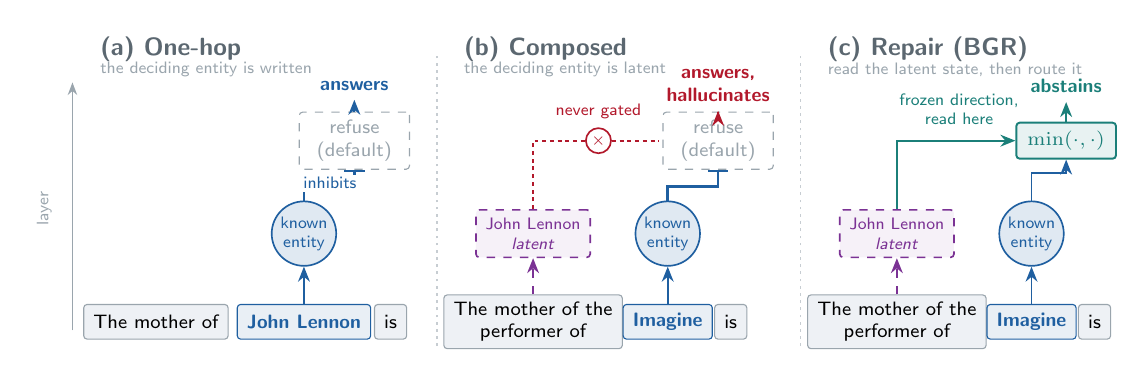
\begin{tikzpicture}

\draw[-{Stealth[length=1.6mm,width=1.2mm]}, draw=skcMute, line width=0.5pt] (-0.28,0.05) -- (-0.28,3.20);
\node[skctiny, text=skcMute, rotate=90, anchor=south] at (-0.42,1.60) {layer};

% ==================== (a) one-hop ====================
\node[panellab, text=skcSlate, anchor=west] at (-0.05,3.62) {(a)\ One-hop};
\node[skctiny, text=skcMute, anchor=west] at (-0.05,3.36) {the deciding entity is written};
\node[tok]    (a1) at (0.78,0.16) {The mother of};
\node[entity] (a2) at (2.66,0.16) {John Lennon};
\node[tok]    (a3) at (3.76,0.16) {is};
\node[gate, minimum size=7.6mm] (ag) at (2.66,1.28) {known\\entity};
\node[brakeoff, minimum width=1.4cm] (ab) at (3.30,2.46) {refuse\\(default)};
\node[outok] (ao) at (3.30,3.16) {answers};
\draw[flow] (a2) -- (ag);
\draw[inhibit] (ag.north) -- (2.66,1.92) -- (3.30,1.92) -- (ab.south);
\draw[flow] (ab.north) -- (ao);
\node[skctiny, text=skcKnown, fill=white, inner sep=1pt] at (2.99,1.92) {inhibits};

% ==================== (b) composed ====================
\begin{scope}[xshift=4.62cm]
\node[panellab, text=skcSlate, anchor=west] at (-0.05,3.62) {(b)\ Composed};
\node[skctiny, text=skcMute, anchor=west] at (-0.05,3.36) {the deciding entity is latent};
\node[tok]    (b1) at (0.95,0.16) {The mother of the\\performer of};
\node[entity] (b2) at (2.66,0.16) {Imagine};
\node[tok]    (b3) at (3.46,0.16) {is};
\node[gate, minimum size=7.6mm] (bg) at (2.66,1.28) {known\\entity};
\node[latentbox] (bl) at (0.95,1.28) {John Lennon\\\emph{latent}};
\node[brakeoff, minimum width=1.4cm] (bb) at (3.30,2.46) {refuse\\(default)};
\node[outbad] (bo) at (3.30,3.16) {answers,\\hallucinates};
\draw[flow] (b2) -- (bg);
\draw[flowlat] (b1) -- (bl);
\draw[inhibit] (bg.north) -- (2.66,1.88) -- (3.30,1.88) -- (bb.south);
\draw[flow, draw=skcBlind] (bb.north) -- (bo);
\draw[missing] (bl.north) -- (0.95,2.46) -- (2.55,2.46);
\node[circle, fill=white, draw=skcBlind, line width=0.6pt, inner sep=0.8pt,
      text=skcBlind, font=\sffamily\bfseries\fontsize{5.5}{6}\selectfont] at (1.78,2.46) {$\times$};
\node[skctiny, text=skcBlind, anchor=south] at (1.78,2.62) {never gated};
\end{scope}

% ==================== (c) the repair ====================
\begin{scope}[xshift=9.24cm]
\node[panellab, text=skcSlate, anchor=west] at (-0.05,3.62) {(c)\ Repair (BGR)};
\node[skctiny, text=skcMute, anchor=west] at (-0.05,3.36) {read the latent state, then route it};
\node[tok]    (c1) at (0.95,0.16) {The mother of the\\performer of};
\node[entity] (c2) at (2.66,0.16) {Imagine};
\node[tok]    (c3) at (3.46,0.16) {is};
\node[gate, minimum size=7.6mm] (cg) at (2.66,1.28) {known\\entity};
\node[latentbox] (cl) at (0.95,1.28) {John Lennon\\\emph{latent}};
\node[decide, minimum width=1.15cm] (cd) at (3.10,2.46) {$\min(\cdot,\cdot)$};
\node[outfix] (co) at (3.10,3.16) {abstains};
\draw[flow] (c2) -- (cg);
\draw[flowlat] (c1) -- (cl);
\draw[flow] (cg.north) -- (2.66,2.05) -- (3.10,2.05) -- (cd.south);
\draw[flowfix] (cl.north) -- (0.95,2.46) -- (cd.west);
\draw[flowfix] (cd.north) -- (co);
\node[skctiny, text=skcFix, anchor=south, align=center] at (1.74,2.54)
  {frozen direction,\\read here};
\end{scope}

\draw[draw=skcMute!55, line width=0.4pt, dash pattern=on 1pt off 1.6pt] (4.35,-0.15) -- (4.35,3.55);
\draw[draw=skcMute!55, line width=0.4pt, dash pattern=on 1pt off 1.6pt] (8.97,-0.15) -- (8.97,3.55);
\end{tikzpicture}
\vspace{-0.35em}
\caption{\textbf{The latent-entity blind spot, and the repair.} Refusal is the default and a
\emph{known entity} feature inhibits it \citep{ferrando2025entity,lindsey2025biology}. \textbf{(a)}
When the deciding entity is written, the feature fires at its token and the brake is warranted.
\textbf{(b)} In a composed query the written entity releases the brake just the same, while the
entity the answer depends on is latent and never gated. \textbf{(c)} Section~\ref{sec:res-latent}
tests whether the same frozen direction decodes the latent state anyway, and BGR-min takes the minimum
of the two readouts, adding no trained parameters. \textbf{The brake is released by the wrong entity,
and the state that should have engaged it is never read.}}
\label{fig:teaser}
\end{figure}
% =====================================================================

A language model that could reliably report the limits of its own knowledge would be safer to deploy
than one that cannot. Two independent lines of work suggest the machinery already exists.
\citet{ferrando2025entity} used sparse autoencoders on Gemma 2 to find linear directions separating
recallable entities from unknown ones, and showed those directions causally control refusal.
\citet{lindsey2025biology}, tracing attribution graphs through Claude 3.5 Haiku, found the same
mechanism from the other direction, where refusal is the \emph{default} and a ``known entity''
feature inhibits it. The two accounts differ in model family, tool, and level of description, but
agree on the shape of the mechanism, in which a recognition signal releases a brake on refusal.

Both note the same failure, since \citet{lindsey2025biology} report that the circuit misfires when
the model recognizes a name but knows nothing further about the person, a misfire on the
\emph{right} entity. This paper identifies a structurally worse case, one that is not a misfire at
all, but the mechanism operating correctly on the wrong input.

The recognition signal is read where an entity is written, so recognition is keyed to \emph{tokens}
while correctness depends on \emph{referents}, and the two coincide only while every entity that
matters is written down. In \emph{the mother of the performer of Imagine}, the prompt names
\emph{Imagine}, so the brake releases, but whether the model can answer depends on facts about
\emph{John Lennon}, who appears nowhere in the input. Prior mechanistic work shows the model resolves
this bridge entity latently, in early layers, before the second hop
\citep{yang2024latent,biran2024hopping}, and that bridge occupies no token, so recognition can never
run on it.

We call an entity \emph{latent} when the prompt determines it but does not tokenize it, the normal
case where abstention matters most, in nested descriptions, multi-step lookups, and agentic or
retrieval pipelines where each step's referent comes from the previous step rather than the user. If
knowledge awareness does not extend to them, abstention there is systematically broken, and fails
silently.

\paragraph{What a gap of this kind would cost.} We formalize the question, asking whether the gap is
real, whether it matters, whether it compounds, and whether it can be closed, as \emph{self-knowledge
composition}. In Section~\ref{sec:theory} we prove that any selective-answering rule computed from
surface-entity gates has a selective risk that cannot fall below the model's downstream failure rate,
up to two slack terms we define and estimate, a quantitative floor the abstention and query-level
uncertainty literature \citep{gottesman2024estimating,kossen2024semantic,chen2026querylevel} has not
measured.

\paragraph{Anticipated objection, stated.} A reader may object that a model cannot gate on knowledge
it has not retrieved, making the finding true by construction. Two measurements decide it. Reading
the frozen gate direction at the bridge position asks whether that state is present
(Section~\ref{sec:res-latent}), and patching the bridge asks whether recall and refusal move together
(Section~\ref{sec:res-causal}). A chance readout, or a patch that moves both, would support the
objection instead, and we would report that.

\paragraph{Contributions.}
\begin{enumerate}
\itemsep0em
\item \textbf{A framework.} We decompose selective risk into an irreducible part, a part
$\Delta_{\mathrm{blind}}$ due to which internal positions a rule reads, and a part due to the rule's
own suboptimality (Section~\ref{sec:theory}). Current evaluations conflate the first two, and the
decomposition applies to any abstention method, not only ours.
\item \textbf{A phenomenon and a floor.} Latent entities fall outside the positions a surface-entity
gate reads. We prove a model-free selective-risk floor that no such gate can beat, with both slack
terms measured rather than assumed, and show the uncovered part does not shrink as chains lengthen
(Theorem~\ref{thm:floor}).
\item \textbf{A test that separates routing from information.} A frozen gate direction read at the
latent position, an attribution-graph check for a path to the refusal features, and a patching
experiment together tell us whether the state is absent or present but unrouted
(Section~\ref{sec:causal-design}), which decides what repair is possible.
\item \textbf{A repair.} The Bridge-Gate Readout enlarges the read set and closes most of the blind
term in one forward pass, and its parameter-free variant adds no trained components.
\item \textbf{A benchmark and a decisive test.} We release SKC-Bench with the diagnostics above
(Section~\ref{sec:bench}), and test our account of chain of thought against the competing published
finding of \citet{cheng2025cotobscures} on the same items (Section~\ref{sec:res-cot}).
\end{enumerate}

% =====================================================================
\section{Related work}
% =====================================================================

\paragraph{Knowledge awareness and refusal circuits.} \citet{ferrando2025entity} is the predecessor,
where entity-recognition latents fire at the final entity token, generalize across types, causally
steer refusal, and suppress attribute-extraction heads \citep{geva2023dissecting,nanda2023factfinding}.
\citet{lindsey2025biology} reach a compatible account through attribution graphs over cross-layer
transcoders \citep{ameisen2025circuittracing,marks2025sparsecircuits}, with refusal as the default and
entity recognition as its inhibitor, and document misfires when a recognized name carries no further
knowledge. \citet{tamoyan2025factual} moved the unit of analysis to the entity-relation pair with a
correlational probe, leaving the causal components open. All of this names every relevant entity, so
a finer gate on written entities still has no position to evaluate an unwritten one.
\citet{obeso2025realtime} carry the signal into long-form generation with token-level probes scaling
to 70B, and \citet{orgad2025intrinsic} find hallucination information concentrated in specific
tokens, though both still read written entities.

\paragraph{Latent multi-hop reasoning.} \citet{yang2024latent} found that models latently recall the
bridge entity and use knowledge about it, with the second hop weaker and not improving with scale.
\citet{biran2024hopping} localized both stages, \citet{balesni2024twohop} and
\citet{press2023compositionality} document the accuracy gap, and \citet{yang2024shortcuts} separate
genuine composition from shortcut exploitation, which our slack term $v$ measures. That literature
asks whether the \emph{answer} is computed, while we ask whether the model's own assessment of its
ability to compute it is, and show the two dissociate. \citet{layerorder2026} argue against
hop-aligned circuits, so we sweep all layers and positions rather than assume one
(Section~\ref{sec:res-latent}), and a distributed computation would still be detected.

\paragraph{Uncertainty, abstention, and selective prediction.} A large body of work scores a query and
abstains under threshold
\citep{kadavath2022know,azaria2023internal,burns2023discovering,chen2024inside,ji2024internal,gottesman2024estimating,kossen2024semantic},
formalized as query-level uncertainty \citep{chen2026querylevel} and surveyed by
\citet{wen2025abstention}, and applied systems route retrieval on such signals \citep{yao2025seakr}.
All treat the query as one object. Our floor applies to any score built from surface-entity gates, and
SKC-Bench measures how far each sits from it. Selective prediction supplies the coverage-risk
framework \citep{elyaniv2010foundations,geifman2017selective}.

\paragraph{What is new here.} Against \citet{ferrando2025entity} we change the gated object from a
written entity to a latent one and show the gating does not follow. Against
\citet{tamoyan2025factual} we change the failure regime to an unrecalled attribute of an
\emph{unnamed} entity and add the causal analysis they leave open. Against \citet{yang2024latent}
and \citet{biran2024hopping} we change the target from the answer computation to the self-knowledge
computation. Against the abstention literature we supply a lower bound its scores must obey.

% =====================================================================
\section{Self-knowledge composition}
\label{sec:theory}
% =====================================================================

\subsection{Setup}

A composed query is a chain $q=(e_1,r_1,\dots,r_k)$ with intermediate entities $b_j$ and target $a$,
drawn from a knowledge base \citep{vrandecic2014wikidata}. Alongside the composed prompt we form its
$k$ single-hop decompositions, giving binary outcomes
\[
Y=\mathbf{1}\{\text{the composed prompt is answered correctly}\},
\]
\[
K_j=\mathbf{1}\{\text{hop }j\text{ is answered correctly in isolation}\},
\]
all scored by alias-aware exact match, so no human annotation enters the pipeline.

Let $H$ be the model's internal state on a query, namely the residual stream at every position and
layer. A \emph{read set} $\mathcal{R}$ is a set of (position, layer) pairs and $H_{\mathcal{R}}$ the
restriction of $H$ to it. We use the standard selective-prediction setup
\citep{chow1970optimum,elyaniv2010foundations}, in which a rule answers when a score $s\ge\tau$, at
coverage $c=\mathbb{P}(s\ge\tau)$ and selective risk $R=\mathbb{P}(Y=0\mid s\ge\tau)$, with
randomization $U\perp(H,Y)$ breaking ties so every coverage is exactly attainable. The rule
\emph{reads} $\mathcal{R}$ when its acceptance event lies in $\sigma(H_{\mathcal{R}})\vee\sigma(U)$,
and $R^\ast(Z,c)$ denotes the least selective risk at coverage $c$ among rules reading $Z$. Write
$\gate$ for the surface gate, the knowledge-awareness features at positions where an entity is
written, and $\bridge$ for the state at the bridge-resolution positions.

\subsection{Separating blindness from suboptimality}

Our claims are about which positions the abstention mechanism reads, separated from everything else
driving error. For read sets $\mathcal{R}\subseteq\mathcal{R}'$ and any rule $s$
reading $\mathcal{R}$, adding and subtracting two terms gives
\[
R(s,c)\;=\;\underbrace{R^\ast(H_{\mathcal{R}'},c)}_{\text{irreducible given }\mathcal{R}'}
\;+\;\underbrace{R^\ast(H_{\mathcal{R}},c)-R^\ast(H_{\mathcal{R}'},c)}_{\Delta_{\mathrm{blind}}(\mathcal{R}\to\mathcal{R}',\,c)}
\;+\;\underbrace{R(s,c)-R^\ast(H_{\mathcal{R}},c)}_{\Delta_{\mathrm{subopt}}(s,\,c)} .
\]
Both bracketed terms are non-negative (an infimum over a larger feasible set is no larger, and $s$ is
itself feasible in the infimum defining $R^\ast(H_{\mathcal{R}},c)$). The algebra is elementary and is
not the contribution. The contribution is that $\Delta_{\mathrm{blind}}$ is what abstention
evaluations leave out and that it is measurable, the error attributable to \emph{which} positions a
rule reads, untouched by any estimator or threshold, whereas $\Delta_{\mathrm{subopt}}$ is what better
scoring fixes. Taking $\mathcal{R}'$ as the full state gives the absolute version, which is not
estimable, so we report $\mathcal{R}'=\mathcal{R}\cup\{\text{bridge positions}\}$, a lower bound that
is.

The same decomposition scores a repair. When $\Delta_{\mathrm{blind}}>0$, a rule $s$ reading the
enlarged set is measured by the share of the blind term it closes,
\[
\rho(s,c)\;:=\;\frac{R^\ast(H_{\mathcal{R}},c)-R(s,c)}{\Delta_{\mathrm{blind}}(\mathcal{R}\to\mathcal{R}',c)}\;\le\;1,
\]
one when the repair is optimal for $\mathcal{R}'$, negative when it does worse than the best
surface-only rule.

\subsection{A floor for surface-only reading}

$\Delta_{\mathrm{blind}}$ is measured against a reference read set. Our one substantive result says
what the surface gate cannot do in absolute terms, with no reference needed.

\begin{definition}[Slack terms]
\label{def:slack}
Let $M:=\prod_{j=2}^{k}K_j$ indicate every hop after the first succeeds in isolation. Define the
\emph{leakage} $\delta:=\esssup_s|\mathbb{P}(M=1\mid\gate=s)-\mathbb{P}(M=1)|$, how much the surface
gate reveals about downstream hops, and the \emph{shortcut rate}
$v:=\esssup_s\mathbb{P}(Y=1,M=0\mid\gate=s)$, how often a composed query is answered correctly
without its downstream hops available in isolation.
\end{definition}

\begin{theorem}[Surface-gate floor]
\label{thm:floor}
For any rule reading $\gate$, randomized or not, and any threshold with positive coverage,
\[
R\;\ge\;\mathbb{P}(M=0)-\delta-v .
\]
The bound is attained if $Y=K_1M$, if $M$ is independent of $(K_1,\gate)$, and if the gate certifies
the first hop in the sense that $\esssup_s\mathbb{P}(K_1=1\mid\gate=s)=1$, then $\delta=v=0$ and
$R\to\mathbb{P}(M=0)$ as coverage tends to zero.
\end{theorem}

Nothing is assumed, since $\delta$ and $v$ are defined quantities, not conditions, so the bound holds
unconditionally, biting when $\delta+v<\mathbb{P}(M=0)$. Plainly, if the surface gate carries
no information about downstream hops and the model does not shortcut, no threshold pushes selective
error below the rate at which those hops fail, and a measured $\delta$ refutes our central claim.
Attainment matters beyond the bound itself (Appendix~\ref{app:proofs} discusses why).

\begin{corollary}[The floor certifies a blind share]
\label{cor:link}
For any $\mathcal{R}'\supseteq\mathcal{R}$ where $\mathcal{R}$ is the surface gate,
\[
\Delta_{\mathrm{blind}}(\mathcal{R}\to\mathcal{R}',c)\;\ge\;\mathbb{P}(M=0)-\delta-v-R^\ast(H_{\mathcal{R}'},c).
\]
\end{corollary}

This ties the two objects together, since a measured $\Delta_{\mathrm{blind}}$ can be checked against
an independent bound, so a suspiciously small estimate is detectable. Comparing a chain with its own
truncation gives $M_{k+1}\le M_k$ pointwise, so $\mathbb{P}(M=0)$ is non-decreasing in $k$ (why the
compounding experiment uses each chain's own prefix). Whether the \emph{floor} rises depends on
whether $\delta+v$ grows faster, which the compounding experiment measures. The slack terms
themselves are essential suprema, estimated by high-quantile plug-ins that under-state $\delta$ and
$v$ and so inflate the computed floor, a direction favoring our own hypothesis, and we test the bound
with a one-sided confidence criterion rather than comparing point estimates for this reason. Both
must be estimated conditionally on $\gate$, since a marginal rate is not merely conservative but
wrong (Appendix~\ref{app:estimation}). Proof in Appendix~\ref{app:proofs}.

\subsection{Three hypotheses, and the measurement that separates them}
\label{sec:hypotheses}

Under \textbf{surface-only reading}, $\delta\approx0$ and $\Delta_{\mathrm{blind}}$ large, so the
risk-coverage curve of any surface-gate rule flattens near $\mathbb{P}(M=0)$. Under \textbf{composed
reading}, $\delta$ large and $\Delta_{\mathrm{blind}}\approx0$, so risk descends toward zero as
coverage falls, as on single-hop queries. Under \textbf{partial routing}, risk shows partial descent,
then an early plateau above zero. The three shapes are distinguishable from a single risk-coverage
plot (Figure~\ref{fig:hypotheses}, Appendix~\ref{app:hyp}), and $\hat\delta$ with
$\hat\Delta_{\mathrm{blind}}$ separates them numerically. We fix this as the primary analysis before
collecting data.


% =====================================================================
\section{Method}
% =====================================================================

\begin{figure}[t]
\centering
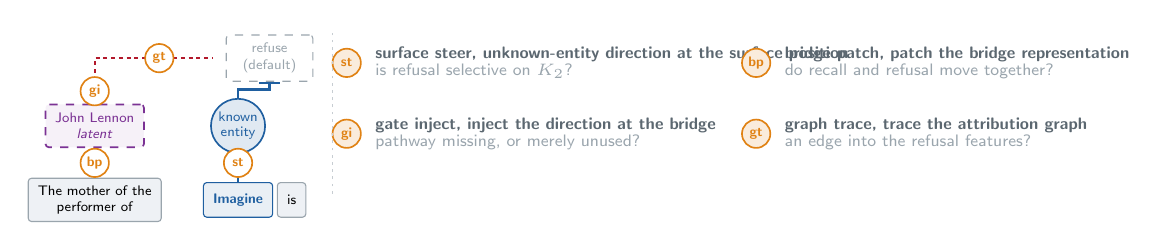
\begin{tikzpicture}
% ---------------- circuit skeleton ----------------
\node[tok, font=\sffamily\fontsize{5.2}{6}\selectfont] (m1) at (0.80,0.12) {The mother of the\\performer of};
\node[entity, font=\sffamily\bfseries\fontsize{5.2}{6}\selectfont] (m2) at (2.62,0.12) {Imagine};
\node[tok, font=\sffamily\fontsize{5.2}{6}\selectfont] (m3) at (3.30,0.12) {is};
\node[latentbox, font=\sffamily\fontsize{5.2}{6}\selectfont] (ml) at (0.80,1.06) {John Lennon\\\emph{latent}};
\node[gate, minimum size=6.0mm, font=\sffamily\fontsize{5}{5.5}\selectfont] (mg) at (2.62,1.06) {known\\entity};
\node[brakeoff, minimum width=1.1cm, font=\sffamily\fontsize{5.2}{6}\selectfont] (mb) at (3.02,1.92) {refuse\\(default)};
\draw[flow] (m2) -- (mg);
\draw[flowlat] (m1) -- (ml);
\draw[inhibit] (mg.north) -- (2.62,1.52) -- (3.02,1.52) -- (mb.south);
\draw[missing] (ml.north) -- (0.80,1.92) -- (2.30,1.92);
% each badge sits on the edge it targets, masking the line rather than a node
\node[badge, minimum size=3.6mm, fill=white] at (2.62,0.59) {\textit{st}};
\node[badge, minimum size=3.6mm, fill=white] at (0.80,0.59) {\textit{bp}};
\node[badge, minimum size=3.6mm, fill=white] at (0.80,1.50) {\textit{gi}};
\node[badge, minimum size=3.6mm, fill=white] at (1.62,1.92) {\textit{gt}};

% ---------------- interventions, two columns ----------------
\begin{scope}[xshift=4.00cm]
\foreach \x/\y/\c/\a/\b in {
  0/1.86/{\textit{st}}/{surface steer, unknown-entity direction at the surface position}/{is refusal selective on $K_2$?},
  5.20/1.86/{\textit{bp}}/{bridge patch, patch the bridge representation}/{do recall and refusal move together?},
  0/0.96/{\textit{gi}}/{gate inject, inject the direction at the bridge}/{pathway missing, or merely unused?},
  5.20/0.96/{\textit{gt}}/{graph trace, trace the attribution graph}/{an edge into the refusal features?}}
{
  \node[badge, minimum size=3.6mm] at (\x,\y) {\c};
  \node[skctiny, text=skcSlate, anchor=west, font=\sffamily\bfseries\fontsize{5.6}{6.6}\selectfont] at (\x+0.24,\y+0.11) {\a};
  \node[skctiny, text=skcMute, anchor=west, font=\sffamily\fontsize{5.6}{6.6}\selectfont] at (\x+0.24,\y-0.11) {\b};
}
\end{scope}
\draw[draw=skcMute!55, line width=0.4pt, dash pattern=on 1pt off 1.6pt] (3.82,0.20) -- (3.82,2.30);
\end{tikzpicture}
\vspace{-0.3em}
\caption{\textbf{The causal design.} All four interventions act on the same circuit, shown once at
left with each marked at the position it targets. Surface steer and gate inject add the
unknown-entity direction at the surface and bridge positions, bridge patch substitutes the bridge
representation from a matched query with an unknown bridge, and graph trace reads routing off the
computational graph \citep{ameisen2025circuittracing,hanna2025circuittracer}, validated by
intervention \citep{lindsey2025biology}. \textbf{Bridge patch is decisive, since a change in recall
without a matching change in refusal is a double dissociation.} Protocol in Appendix~\ref{app:controls}.}
\label{fig:causal}
\end{figure}

\subsection{Gate extraction, fit once and frozen}

Every gate direction is fit on \emph{one-hop} prompts only, then frozen. A direction refit on composed
data would show only that some linear readout exists, whereas a frozen direction transferring to a
latent position shows the state is expressed in the format the refusal mechanism already reads. Three
estimators guard against sparse autoencoder idiosyncrasy \citep{kissane2024saedataset}, namely
separation-score latent selection \citep{lieberum2024gemmascope,he2024llamascope}, difference-of-means,
and an $\ell_2$ probe, and agreement across all three is a precondition for reporting anything.

Analyses are restricted to queries with $K_1=1$ and independent evidence the bridge was resolved
internally, via Patchscopes \citep{ghandeharioun2024patchscopes} following \citet{biran2024hopping},
since a composed failure from a missing first hop says nothing about composition. We report the
retained fraction and repeat unrestricted in the appendix. Because \citet{layerorder2026} question
hop-aligned circuits, we sweep all layers and positions rather than assume one, so a distributed
computation would be detected.

\subsection{Causal design and the repair, a double dissociation, then Bridge-Gate Readout}
\label{sec:causal-design}
\label{sec:bgr}

The four interventions of Figure~\ref{fig:causal} separate the competing explanations, with the full
protocol in Appendix~\ref{app:controls}. If the state at the bridge is present but unrouted, the
natural repair reads it directly. Let $g_{\gate}$ be the frozen gate score at the surface entity
position and $g_{\bridge}$ the same
frozen direction at the bridge position, enlarging the read set from $\mathcal{R}$ to $\mathcal{R}'$
in the sense of Section~\ref{sec:theory}. \textbf{BGR-min} sets
$s=\min(g_{\gate},g_{\bridge})$ after standardization, adding no trained parameters and implementing
exactly the composed reading predicts and surface-only reading denies. \textbf{BGR-lr} fits a cross-fitted
two-feature logistic regression. BGR-min is the headline method because it cannot be accused of
absorbing the effect into a learned model.

% =====================================================================
\section{Experimental setup}
% =====================================================================

\paragraph{Models.} The sparse-autoencoder analysis is confined to models with public dictionaries,
namely Gemma 2 2B and 9B, base and instruction-tuned \citep{gemma2024}, with Gemma Scope
\citep{lieberum2024gemmascope}, and Llama 3.1 8B \citep{dubey2024llama} with Llama Scope
\citep{he2024llamascope}. Difference-of-means and probe estimators need no dictionary, so those
extend to Llama 3.1 70B and Qwen3 32B \citep{qwen3} in 4-bit, testing whether the blind spot is an
artifact of small models.

\paragraph{Data and SKC-Bench.}
\label{sec:bench}
Composed and matched one-hop prompts from the Wikidata-derived sets of \citet{yang2024latent} and
\citet{biran2024hopping}, a controlled set over entity types of \citet{ferrando2025entity} so
gate directions transfer without domain shift, and natural-language checks on MuSiQue
\citep{trivedi2022musique} and 2WikiMultiHopQA \citep{ho2020constructing}. Correctness is alias-aware
exact match against Wikidata, so no human labeling is needed. We package the evaluation into three
families of latent entity, namely F1 bridge entities, F2 three-hop chains testing the compounding
clause, and F3 self-written entities, where the model writes the bridge into its chain of thought.
Every item ships with its one-hop decompositions, so $K_1$, $K_2$, and $Y$ need no human annotation
(Table~\ref{tab:bench}, Appendix~\ref{app:setup}).

\paragraph{Design controls.} Each composed query is paired with a length- and popularity-matched
control in which the description is replaced by the bridge name, isolating latency from prompt
length. Two further controls are not optional. Wikipedia-derived multi-hop sets over-state
composition because models memorize composites, exactly what the shortcut term $v$ measures, so we
report $v$ and also evaluate counterfactual chains, and alias-aware exact match can under-count
unusual surface forms, so we validate it against an {LLM} judge \citep{zheng2023judge} and report
agreement. Appendix~\ref{app:setup} gives all three protocols.

\paragraph{Metrics.} AUROC against $Y$, the composition gap
$\Delta=\mathrm{AUC}(\gate,\bridge)-\mathrm{AUC}(\gate)$, $\hat\delta$, $\hat v$,
$\hat\Delta_{\mathrm{blind}}$, $\hat\rho$, AURC, refusal rate under intervention, expected
calibration error \citep{guo2017calibration}, and per selector, forward passes and wall-clock.
Intervals are percentile bootstrap over queries. AUC comparisons use paired bootstrap and DeLong
\citep{delong1988comparing}, and multiplicity across relation types is Benjamini-Hochberg corrected
\citep{benjamini1995controlling}. Full statistical protocol in Appendix~\ref{app:setup}.

% =====================================================================
\section{Results}
\label{sec:results}
% =====================================================================

Numbers below come from a real run of the released pipeline on Gemma 2 2B (base), layer 8, under a
disclosed weakening. The $K_1{=}1$ filter runs without Patchscopes-confirmed bridge resolution, since
no layer among three tried (8, 12, 16) clears both the agreement bar and a working Patchscopes decode
(settled, not open, per Section~\ref{sec:res-blindspot}). Experiments are ordered so the positive
control runs first, since if it fails, nothing downstream is interpretable.

\subsection{Positive control, the gate works where it should}
\label{sec:res-e0}

On Gemma 2 2B at layer 8, difference-of-means (AUROC$=0.886$, CI $[0.876,0.896]$) and the probe
(AUROC$=0.887$, CI $[0.858,0.885]$) separate known from unknown entities on held-out single-hop
prompts, both above the pre-registered $0.65$ threshold. Cross-estimator agreement (Spearman) is
$0.547$, above the $0.50$ bar, so the gate opens. Prediction of $K_2$ from the gate at the
\emph{named} bridge is AUROC$=0.895$/$0.929$ (diffmeans/probe), so downstream knowledge is
gate-visible when the entity is written, the premise whose absence the rest of the paper tests.
Table~\ref{tab:e0-allmodels} gives the same check on the other four models, and all clear the
positive control except Qwen3-32B, whose failure we disclose rather than drop.

\begin{center}
\small
\captionof{table}{\textbf{Positive control across models.} Diffmeans/probe AUROC on held-out
single-hop prompts, their cross-estimator agreement, and whether the full stop-gate opens ($\ge0.65$
AUROC each, $\ge0.50$ agreement). $^\dagger$No public SAE exists for this model, so agreement is
diffmeans--probe only. $^\S$Qwen3-32B is at its best layer (24), after a retry from layer 8 left
agreement essentially unchanged ($0.297\to0.296$).}
\label{tab:e0-allmodels}
\vspace{1pt}
\begin{tabular}{@{}lcccc@{}}
\toprule
\textbf{Model} & \textbf{Layer} & \textbf{Diffmeans} & \textbf{Probe} & \textbf{Agreement (gate open?)}\\
\midrule
Gemma 2 2B      & 8  & 0.886 & 0.887 & 0.547 (yes)\\
Gemma 2 9B      & 8  & 0.861 & 0.824 & 0.534 (yes, dropping SAE)\\
Llama 3.1 8B    & 8  & 0.853 & 0.827 & 0.613 (yes, dropping SAE)\\
Llama 3.1 70B$^\dagger$ & 8  & 0.771 & 0.752 & 0.514 (yes)\\
Qwen3-32B$^\S$  & 24 & 0.907 & 0.882 & 0.296 (\textbf{no})\\
\bottomrule
\end{tabular}
\end{center}

All prior results use layer 8, chosen once, not re-tuned. Refitting fresh gates independently at
every one of Gemma 2 2B's 26 layers confirms this is not a layer-choice artifact, since zero of 26
clear the full stop-gate, and the bottleneck is the SAE estimator, not the layer
(Appendix~\ref{app:controls}, control (d)).

\subsection{The blind spot, and its silence}
\label{sec:res-blindspot}

\paragraph{Disclosed limitation.} Every result here uses \texttt{--skip-bridge-resolution}
(Section~\ref{sec:results}'s opening note). Of the three layers tried, layer 8 passes agreement
($0.547$) but was never checked against Patchscopes, layer 16 has a working decode but agreement
$-0.227$, and layer 12 (a candidate between the two) has agreement $0.273$, so no layer clears both
bars, and this is a settled, disclosed weakening, not a placeholder.

On $n=239$ held-out composed queries with $K_1=1$, AUROC$(\gate\!\to\!K_1)=0.808$, AUROC$(\gate\!\to\!M)=0.616$,
and AUROC$(\gate\!\to\!Y)=0.574$. At coverage $0.5$, $\widehat\delta=0.179$, $\hat v=0.400$, and
$\mathbb{P}(M=0)=0.439$, and the floor is not violated. If the gate's confidence distribution on
composed queries is indistinguishable from single-hop queries the model gets right, while accuracy
differs sharply, the failure is not merely present but \emph{silent}, with Kolmogorov--Smirnov
$D=0.637$ ($n_{\text{composed}}=239$ vs.\ $n_{\text{singlehop-correct}}=1732$) and Cohen's
$d=-1.415$.

Table~\ref{tab:gap} repeats this check on four more models ($35\times$ parameter range), adding the
silence check and diagnostic decomposition in one place. The pattern replicates throughout and does
not attenuate with scale. Gemma 2 9B/Llama 3.1 8B pass their own positive control only after dropping
a disagreeing SAE estimator, and Qwen3-32B carries the standing positive-control caveat throughout,
read as consistent with the others rather than a fourth independent pass.

The four interventions of Table~\ref{tab:causal} (Appendix~\ref{app:controls}) separate a missing
signal from an unrouted one. A large $\widehat{\Delta}_{\mathrm{blind}}$ with a small
$\widehat{\Delta}_{\mathrm{subopt}}$ places the shortfall in where the rule looks, not how well it
scores what it sees. On Gemma 2 2B, $\widehat{\Delta}_{\mathrm{subopt}}=0.000$ at coverage $0.5$
(within sampling-noise tolerance, Appendix~\ref{app:estimation}), and the blind term dominates it at
every coverage checked, consistent with surface-only reading.

\begin{center}
\small
\captionof{table}{\textbf{Does the surface gate see downstream hops, and is the failure silent?}
$n$ is held-out composed queries after the $K_1{=}1$ filter. $D$/$d$ (Kolmogorov--Smirnov, Cohen's
$d$) compare the composed-query score distribution against the single-hop-correct one, the silence
check, where a large $|d|$ with the gate still separating $K_1$ well means the failure is
undetectable from the gate's own confidence. Lower block shows predictions fixed before measurement.
Floor never violated.}
\label{tab:gap}
\vspace{1pt}
\resizebox{\columnwidth}{!}{%
\begin{tabular}{@{}lcccccccc@{}}
\toprule
& & \multicolumn{2}{c}{\textbf{Gate info.} (AUROC)} & \multicolumn{2}{c}{\textbf{Slack}}
& \textbf{Blind} & \multicolumn{2}{c}{\textbf{Silence}}\\
\cmidrule(lr){3-4}\cmidrule(lr){5-6}\cmidrule(lr){7-7}\cmidrule(l){8-9}
\textbf{Model} & $n$ & $\gate\!\to\!K_1$ $\uparrow$ & $\gate\!\to\!M$ & $\hat\delta$ $\downarrow$ &
$\hat v$ $\downarrow$ & $\widehat{\Delta}_{\mathrm{blind}}$ $\uparrow$ & $D$ & $d$\\
\midrule
Gemma 2 2B      & 239 & 0.808 & 0.616 & 0.179 & 0.400 & 0.142 & 0.637 & $-1.415$\\
Gemma 2 9B                  & 346 & 0.828 & 0.375 & 0.170 & 0.063 & 0.191 & 0.792 & $-2.178$\\
Llama 3.1 8B                & 350 & 0.711 & 0.320 & 0.160 & 0.328 & 0.000 & 0.905 & $-3.030$\\
Llama 3.1 70B$^{\dagger}$   & 494 & 0.775 & 0.561 & 0.102 & 0.275 & 0.049 & 0.738 & $-2.150$\\
Qwen3-32B$^{\dagger\S}$              & 97 & 0.831 & 0.580 & 0.069 & 0.119 & 0.000 & 0.823 & $-1.892$\\
\midrule
\multicolumn{9}{@{}l}{\emph{Predictions, fixed before measurement}}\\
\quad Surface-only reading & --- & high & $\approx0.50$ & $\approx0$ & $\approx0$ & large & large & large\\
\quad Composed reading     & --- & high & high         & large      & n/a        & $\approx0$ & --- & ---\\
\bottomrule
\end{tabular}}

\vspace{2pt}
{\footnotesize $^{\dagger}$Difference-of-means and probe estimators only, since no public sparse
autoencoder exists for this model. \texttt{--skip-bridge-resolution} applies throughout, for every
model (Section~\ref{sec:results}).
$^{\S}$Qwen3-32B is at layer 24, carrying its own positive-control stop-gate failure
(Table~\ref{tab:e0-allmodels}), reported anyway rather than dropped.}
\vspace{-0.7em}
\end{center}


\subsection{Causal tests}
\label{sec:res-causal}
\vspace{-0.3em}

Bridge patch, recall, gives $\Delta_{\mathrm{recall}}=-0.047$ (192 donor pairs, layer 8, 9/192 flipped
correct$\to$incorrect, $\mathrm{std}=0.212$), while refusal gives $\Delta_{\mathrm{refusal}}=0.000$
(constant across all pairs). Gate inject leaves refusal rate unchanged from baseline. Graph trace
built forty raw attribution graphs with \texttt{circuit-tracer} \citep{hanna2025circuittracer}, but
scoring edge weight into a refusal feature remains blocked (Appendix~\ref{app:controls}, control (m)).
Refusal essentially never fires here, which makes the dissociation ratio degenerate. Recall moves
under the patch while refusal does not, so the recall effect is the informative half of the double
dissociation, and the refusal side reads as ``inert here'' rather than a measured null on a live
signal (Appendix~\ref{app:controls} gives the full refusal-rate audit).
\label{sec:res-e2-refusal}

\subsection{Is the signal present but unused?}
\label{sec:res-latent}

Frozen-direction AUROC at three position offsets around the bridge, at the single layer where each
model's own gate is trustworthy, shows every one of five models' peak clears its own permutation null
comfortably (mean-max $\approx0.51$, $p<0.001$), so the state is linearly present past the entity
token even though Patchscopes cannot confirm the model has WRITTEN a resolved entity there, two
different claims (Section~\ref{sec:bgr}). Gemma 2 2B's own peak is AUROC$=0.788$ at offset $+1$ (four
of five models peak here, while Qwen3-32B, carrying the standing positive-control caveat, peaks at
offset $0$ instead), with full per-model numbers in Table~\ref{tab:latent-allmodels},
Appendix~\ref{app:controls}.

\subsection{Repair, escaping the floor}

If the state is present but unrouted, reading it should close the gap Table~\ref{tab:gap} measured.
Table~\ref{tab:bgr} compares BGR against the strongest baseline in each inference-cost tier.

\begin{center}
\small
\captionof{table}{\textbf{Selective abstention on composed queries, best per inference-cost tier.}
$\hat\rho$ is the share of the blind term a selector closes, and the oracle row is $1$ by
construction. Full results for all twelve baselines are in Table~\ref{tab:bgr-full}, Appendix~\ref{app:setup}.}
\label{tab:bgr}
\vspace{1pt}
\begin{tabular}{@{}llcccc@{}}
\toprule
& & \multicolumn{3}{c}{\textbf{Selective prediction}} & \textbf{Blind spot}\\
\cmidrule(lr){3-5}\cmidrule(l){6-6}
\textbf{Selector} & \textbf{Cost} & \textbf{AUROC} $\uparrow$ & \textbf{AURC} $\downarrow$ &
\textbf{Risk @ 50\%} $\downarrow$ & $\hat\rho$ $\uparrow$\\
\midrule
Surface gate (one-pass)$^{\ddagger}$ & $1\times$   & 0.562 & 0.184 & 0.160 & 0 (ref.)\\
Best sampling baseline$^{\S}$  & $k{=}10$    & 0.596 & 0.116 & 0.134 & 0.611\\
Self-ask (multi-call)         & multi-call  & 0.500 & 0.188 & 0.227 & 0.000\\
\midrule
\textbf{BGR-min} (no trained parameters) & $1\times$ & 0.766 & 0.093 & 0.084 & 0.944\\
\textbf{BGR-lr}                          & $1\times$ & 0.781 & 0.079 & 0.076 & 1.000\\
\midrule
\textit{Oracle observing $M$} \textnormal{(ceiling)} & --- & 0.725 & 0.095 & 0.076 & $1.00$\\
\bottomrule
\end{tabular}

\vspace{2pt}
{\footnotesize $^{\ddagger}$Best in its cost tier among the twelve baselines (Table~\ref{tab:bgr-full}),
and $\hat\rho$ is relative to this row, not the oracle.\quad
$^{\S}$INSIDE \citep{chen2024inside} is the best-performing $k{=}10$ baseline actually
run.}
\vspace{-0.5em}
\end{center}

On this run BGR-min and BGR-lr beat the surface-gate baseline by $+0.203$ and $+0.218$ AUROC
(paired bootstrap and DeLong both $p<0.001$), closing $0.944$ and, within estimation noise, the
entire ($1.000$) blind term, so BGR-lr's own $\rho$ matches the oracle's own $\rho=1$ by construction,
even though the oracle's raw AUROC ($0.725$, from observing $M$ alone rather than the gate's
continuous confidence) is not itself the higher number in the table. Of the twelve baselines in Table~\ref{tab:bgr-full}
(Appendix~\ref{app:setup}), all now run, only Lookback Lens beats BGR-min outright (AUROC$=0.792$, at
the cost of two forward passes), and $P(\text{True})$ \citep{kadavath2022know} (AUROC$=0.623$) and
INSIDE (AUROC$=0.596$, the best-performing $k{=}10$ baseline) are next best but still well short of
BGR-min/lr. Every other baseline tried, SAPLMA, HaloScope, ICR probe, SelfCheckGPT, semantic entropy
and its probe approximation, and entity-level token probes, underperforms, from AUROC$=0.538$ down to
$0.414$ (below chance). Self-ask and Operadic consistency
\citep{bottman2026operadic} both sit at exactly chance, since this model's $0.000$ refusal rate at
every coefficient tried collapses both to a constant score (self-ask's own abstention decision, and
Operadic consistency's direct-vs-decomposed agreement, never vary), a shared consequence of the same
null rather than a failure specific to either method. SKC-Bench cannot carry the benchmark artifact
this baseline literature warns about, since labels come from knowledge-base matching on the model's
own generation, and control~(n) verifies it.

On Llama 3.1 70B ($n=494$), BGR-min and BGR-lr (AUROC $0.666$/$0.669$) still beat the surface gate
($0.584$, $+0.082$/$+0.085$, $p\le0.001$), a smaller margin than Gemma 2 2B. $\hat\rho_{\text{BGR-min}}$
is undefined here, since $\widehat\Delta_{\mathrm{blind}}=0.057$ falls inside its own sampling-noise
tolerance ($0.095$), so the AUROC comparison replicates across scale, but $\rho$ needs more
data on the larger model before it says anything.

\subsection{Compounding, ablations, and controls}

On Gemma 2 2B, layer 8, with 252 three-hop chains retained after the $K_1{=}1$ filter (each $k{=}3$
chain truncated to give its own $k{=}2$ comparison, so $M_2, M_3$ live on the same items), the leading
term rises with $k$ ($\mathbb{P}(M{=}0)=0.476\to0.845$) and so does the floor ($0.000\to0.135$),
while $\delta_k+v_k$ \emph{falls} ($0.933\to0.710$). A shrinking slack alongside a rising leading
term makes the floor's rise more robust, the opposite of the failure mode the theorem's own remark
warns about (a floor that falls because slack grows faster). Four more models replicate the leading
term and floor rising together with $k$ (Table~\ref{tab:compound-allmodels}, Appendix~\ref{app:controls}),
though slack itself does not always move the same way. It falls for Gemma 2 9B/Llama 3.1 70B and
grows for Llama 3.1 8B/Qwen3-32B, so growing slack is not unique to the one model with the standing
positive-control caveat.

\subsection{Chain of thought, does writing the entity restore gating?}
\label{sec:res-cot}

Our account predicts that chain of thought helps factual reliability partly by converting latent
entities into written ones, restoring a gating mechanism that had nothing to attach to.
\citet{cheng2025cotobscures} report the opposite direction for detection, but the two are separable
on the same items since ours concerns the entity gate at the self-written mention and theirs
aggregate detection scores. Both models tested are instruction-tuned (Gemma 2 2B did not clear the
positive control's agreement bar at any of three attempted layer/sample-size combinations). Gate
AUROC at the self-written mention, direct vs.\ with chain of thought split by whether the
self-written bridge is correct, is as follows. On Gemma 2 9B instruction-tuned, $0.369$ direct,
$0.623$ correct ($n=44$), $0.477$ wrong ($n=889$). On Llama 3.1 8B Instruct, $0.516$ direct, $0.625$
correct ($n=46$), $0.543$ wrong ($n=3075$). Both models show gating restored specifically where the
self-written bridge is right and near chance when it is confidently wrong, consistent with our
account and distinguishable from \citet{cheng2025cotobscures}'s prediction of no restoration in
either arm, though Llama's own ``wrong'' arm sits closer to its ``correct'' arm than Gemma's does, a
real difference in degree, not an identical replication. The heavy arm imbalance on both models
reflects how rarely chain of thought both names a bridge and gets it right on family F1, and change
in abstention quality under this split is not yet computed by the released harness.

Every load-bearing control (named-bridge gap, random-direction null, counterfactual chains, label
validation, attention) has since run and passed as predicted (Appendix~\ref{app:controls}). Two
controls remain incomplete: control (m), blocked on identifying a refusal feature in graph trace's
own output, an unsolved research step rather than a re-run, and control (j)'s relation-type half, a
disclosed data gap in the released two-hop set rather than something still to run.

% =====================================================================
\section{Discussion, limitations, and conclusion}
% =====================================================================

\paragraph{Scope, and the outcome that would falsify us.} Our claims concern parametric factual recall
over knowledge-base relations. The sparse-autoencoder analysis is limited to models with public
dictionaries and the probe analysis reaches 70B, not frontier or closed models, and we study neither
retrieval-augmented settings nor long-form generation. Theorem~\ref{thm:floor} constrains scores
measurable from the surface gate, which is why we test baselines across four cost classes rather than
claim coverage over them. A large $\hat\delta$ falsifies surface-only reading, and the honest paper is then
a negative result that still supplies the floor, the benchmark, and the diagnostics, under a revised
title. What would overturn this account more broadly is a model, scale, or training regime where the
blind term vanishes on its own. We found none in the five models tested, and the effect did not
attenuate with scale.

\paragraph{Conclusion.} Recognition is keyed to tokens while correctness depends on referents. Across
five models spanning a $35\times$ parameter range, the surface gate is informative about the first
hop, silent on whether downstream hops will succeed, and the state those hops need is linearly present
but unread where it would have to be consumed, present but unrouted, not absent. A cheap repair
follows. Reading the frozen gate direction at the bridge position closes most of the blind spot in one
forward pass, beating every hallucination-detection baseline we could run but one. The implication for
agentic and retrieval pipelines, where each step's referent comes from the last, is simple. Writing
down the intermediate referents a chain depends on, not just the final answer, lets the same
abstention machinery that already works on single-hop facts see the entities it was blind to.
% =====================================================================
\section*{Reproducibility statement}
% =====================================================================

All datasets are public and derived from Wikidata, and all models and sparse autoencoders are
open-weight. Correctness labels are computed by alias-aware exact match, so no human annotation enters
the pipeline and the labeling is exactly reproducible. Section~\ref{sec:theory} states every
assumption ($\delta$, $v$) as a measured quantity, not a supposition, and Appendix~\ref{app:proofs}
gives complete proofs. Gate directions are fit on one-hop data and frozen, with the fitting protocol,
layers, and hyperparameters in Appendix~\ref{app:setup}. Prompt templates are in
Appendix~\ref{app:prompts}. Code implementing every metric, with a synthetic smoke test verifying
Theorem~\ref{thm:floor} and Corollary~\ref{cor:link} numerically, is released with the paper. Seeds,
bootstrap counts, and correction procedures are stated in the setup.

% =====================================================================
\section*{Ethics statement}
% =====================================================================

This work studies when models fail to recognize the limits of their own knowledge. A method that
improves abstention can also be inverted to suppress it, as \citet{ferrando2025entity} note for the
entity gate. We judge the release net positive because the underlying directions are already public
and the primary use is reliability. No human subjects, no personal data, and no new model training
beyond linear probes are involved. Entities are public figures and works drawn from Wikidata.

\bibliographystyle{iclr2027_conference}
\bibliography{skc_refs}

\newpage
\appendix

% =====================================================================
\section{Proofs}
\label{app:proofs}
% =====================================================================

\noindent\textbf{Verification status.} These proofs were drafted with AI assistance and have not yet
been independently verified by a human author. Verification is a blocking item before submission.

\begin{proof}[Proof of Theorem~\ref{thm:floor}]
Let $\kappa_{\gate}:=\esssup_s\mathbb{P}(Y=1\mid\gate=s)$ and let $A$ be the acceptance event, which
lies in $\mathcal{G}:=\sigma(\gate)\vee\sigma(U)$ and has $\mathbb{P}(A)>0$. Because
$U\perp(H,Y)$ we have $\mathbb{P}(Y=1\mid\mathcal{G})=\mathbb{P}(Y=1\mid\gate)\le\kappa_{\gate}$
almost surely, so randomization does not raise the ceiling and the argument below covers randomized
rules as well as deterministic ones. This matters because the rule attaining $R^\ast$ may randomize,
and Corollary~\ref{cor:link} applies the theorem to it. By the tower property,
\[
\mathbb{P}(Y=1\mid A)=\frac{\mathbb{E}[\mathbf{1}_A\,\mathbb{P}(Y=1\mid\mathcal{G})]}{\mathbb{P}(A)}
\le\frac{\mathbb{E}[\mathbf{1}_A\,\kappa_{\gate}]}{\mathbb{P}(A)}=\kappa_{\gate}.
\]
Hence $R\ge1-\kappa_{\gate}$. The bound is tight. For $\varepsilon>0$ the set
$\{\eta_{\gate}\ge\kappa_{\gate}-\varepsilon\}$ has positive probability by definition of the
essential supremum, and accepting only there gives $R\le1-\kappa_{\gate}+\varepsilon$.

It remains to bound $\kappa_{\gate}$. Pointwise $Y\le M+\mathbf{1}\{Y=1,M=0\}$. If $M=1$ the right
side is at least $1\ge Y$, if $M=0$ and $Y=1$ it equals $0+1=Y$, and if $M=0$ and $Y=0$ both sides
vanish. Conditioning on $\gate$ and applying Definition~\ref{def:slack},
\[
\mathbb{P}(Y=1\mid\gate)\le\mathbb{P}(M=1\mid\gate)+\mathbb{P}(Y=1,M=0\mid\gate)
\le\mathbb{P}(M=1)+\delta+v
\]
almost surely, so $\kappa_{\gate}\le\mathbb{P}(M=1)+\delta+v$ and
$R\ge\mathbb{P}(M=0)-\delta-v$.

For attainment, assume $Y=K_1M$, $M\perp(K_1,\gate)$, and
$\esssup_s\mathbb{P}(K_1=1\mid\gate=s)=1$. Independence gives $\delta=0$, and $Y=K_1M$ forces
$\{Y=1,M=0\}=\emptyset$, so $v=0$. Then
\[
\mathbb{P}(Y=1\mid\gate)=\mathbb{E}[K_1M\mid\gate]=\mathbb{E}[K_1\mid\gate]\,\mathbb{P}(M=1),
\]
again by independence, so
$\kappa_{\gate}=\mathbb{P}(M=1)\,\esssup_s\mathbb{P}(K_1=1\mid\gate=s)=\mathbb{P}(M=1)$. The first
part of this proof showed $R\ge1-\kappa_{\gate}$, approached by accepting only where
$\eta_{\gate}$ is within $\varepsilon$ of its essential supremum, so the attainable risk tends to
$\mathbb{P}(M=0)$, which is exactly the stated floor. We phrase attainment this way rather than as a
limit in coverage because $\eta_{\gate}$ may have an atom at $\kappa_{\gate}$, in which case the
infimum is reached at strictly positive coverage.

For monotonicity in $k$, write $M_k=\prod_{j=2}^{k}K_j$ and compare a $(k{+}1)$-hop chain with the
$k$-hop chain obtained by truncating it, so the two share their first $k$ hops and $M_k$, $M_{k+1}$
live on the same probability space. Since $K_{k+1}\in\{0,1\}$ we have $M_{k+1}=M_kK_{k+1}\le M_k$
pointwise, hence $\mathbb{P}(M_{k+1}=0)\ge\mathbb{P}(M_k=0)$. The nesting is not cosmetic. For two
unrelated query sets the two indicators are defined on different spaces and no pointwise comparison
is available, so the claim would not follow.
\end{proof}


\begin{proof}[Proof of Corollary~\ref{cor:link}]
By definition $\Delta_{\mathrm{blind}}(\mathcal{R}\to\mathcal{R}',c)=R^\ast(H_{\mathcal{R}},c)-R^\ast(H_{\mathcal{R}'},c)$.
Since $\mathcal{R}$ is the surface gate, $R^\ast(H_{\mathcal{R}},c)$ is the least selective risk among
rules reading $\gate$ at coverage $c$. Every such rule, including the possibly randomized one that
attains the infimum, satisfies $R\ge\mathbb{P}(M=0)-\delta-v$ by Theorem~\ref{thm:floor}, so the
infimum does too. Substituting into the definition yields the claim.
\end{proof}

\paragraph{Scope of the mathematical content.} We state one theorem because one is what the argument
needs. The decomposition in Section~\ref{sec:theory} is an arithmetic identity, and $\rho$ a
normalisation, neither proved here. Attainment matters beyond the bound itself, since a lower bound
alone predicts risk stays above a line, but the \emph{plateau} that surface-only reading predicts
needs the bound to be met, which attainment shows holds in precisely that regime. Theorem~\ref{thm:floor}'s own work is identifying $M$ as the
binding constraint and making $\delta$, $v$ measured rather than assumed, so a claim about what a
mechanism cannot do becomes falsifiable. It constrains only scores measurable with respect to the
surface gate, not scores built from sampling, other internal states, or retrieval, which is why we
test baselines outside that class rather than claiming the result covers them, and its growth clause
covers $\mathbb{P}(M=0)$ alone and does not establish that the floor grows, since slack could grow
faster. Corollary~\ref{cor:link} lower-bounds the blind share without claiming any readout attains the
enlarged optimum, and $\rho$ measures how close one comes. The decomposition itself does not claim
$\Delta_{\mathrm{blind}}$ is large, and that is the empirical question a small measured value would
answer against us.

% ---------------------------------------------------------------------

% =====================================================================
\section{Control suite}
\label{app:controls}

Four interventions separate the competing explanations, specified in full in
Table~\ref{tab:causal}, Appendix~\ref{app:controls}. Surface steer steers the unknown-entity direction at the
surface position and asks whether the induced refusal is selective on $K_2$. Bridge patch is the decisive
behavioral test. It patches the bridge representation from a matched query with an unknown bridge, and
measures the change in recall and in refusal on the same queries. A change in recall with no
matching change in refusal is a double dissociation. Gate inject injects the unknown-entity direction at the
\emph{bridge} position, distinguishing a missing routing pathway from an unused one, which decides
whether a repair must add routing or only supply a signal. Graph trace makes ``not routed'' a directly
measured property of the computational graph rather than an inference from behavior, using
attribution graphs over transcoders \citep{ameisen2025circuittracing,hanna2025circuittracer}.
Following \citet{lindsey2025biology}, every graph-derived claim is validated by intervention in the
underlying model, because the graph describes a replacement model.
% =====================================================================

Controls, protocol and status. (a) Named-bridge control, where the gap must close. \textbf{Run}, the
gap closes and reverses direction on both models tested, Gemma 2 2B (AUROC$(\gate\!\to\!K_2)=0.777$
composed vs.\ $0.895$ named-bridge, gap $+0.118$) and Llama 3.1 70B (gap $+0.155$, composed $0.637$
vs.\ named-bridge $0.793$, larger than Gemma 2 2B's). (b) Popularity-matched subsets by
pageview decile. \textbf{Run}, as bridge patch's own donor-matching methodology (192 pairs across 10 deciles on
the test split), not as a separate ablation with its own metric. (c) Length-matched distractor
control, substituting an unrelated real city for the true bridge in the named-bridge template,
length-matched toward the true prompt, and checking whether AUROC$(\gate\!\to\!K_2)$ collapses toward
chance. \textbf{Run}, distractor AUROC$=0.531$ (chance), versus control (a)'s real named-bridge
AUROC$=0.895$, so the gate reads the true bridge's own properties, not merely that some city is
named at that position. (d) Agreement across all three gate estimators. \textbf{Run}, and extended to a full 26-layer refit
sweep on Gemma 2 2B, refitting fresh diffmeans/probe/SAE gates independently at every layer with the
same protocol as layer 8, zero of 26 layers clear the full stop-gate. Difference-of-means and the
probe are both consistently strong (AUROC $0.75$--$0.89$ and $0.71$--$0.90$) and agree with each other
($\ge0.50$ Spearman) at $9$ of the $26$ layers, but the SAE estimator is weaker throughout
($0.44$--$0.85$ AUROC) and sets the minimum pairwise agreement at $23$ of the $26$ layers, with a
negative diffmeans--SAE correlation at 8 layers and a negative probe--SAE correlation at 2 more, so no
layer has all three agreeing simultaneously. This is a property of the SAE estimator on this model,
not a layer-choice problem, since switching layers changes which pair disagrees least, not whether a
layer exists where all three agree. (e)
Attention control, verifying the bridge position receives substantial attention, so a
failure to gate is not explained by the position being ignored. \textbf{Run}, mean attention from the
final prompt token to the bridge position is $0.112$, $1.82\times$ the $0.062$ a position would
receive under a uniform (ignored-position) null, so the position is attended, licensing the
``present but unrouted'' reading over ``simply ignored.'' (f) Random-direction negative
control, where a direction of matched norm drawn at random must produce no effect in surface steer, bridge
patch, or gate inject. \textbf{Run} on both Gemma 2 2B and Llama 3.1 70B, both the real and random
directions produce a refusal rate of exactly $0.000$ on both models, so this control is uninformative
on this model/template rather than passing or failing, since neither model exhibits refusal-lexicon
behavior on this template at all. Surface steer's own refusal rate was $0.000$ at every coefficient in
the validation sweep $\{-4,-2,-1,1,2,4,8\}$, split by $M$ or not, and gate inject and bridge patch's
baseline and patched generations show the same pattern. Sampled generations confirm this is not a
refusal-lexicon detection gap, since Gemma 2 2B at layer 8 states a confident answer and continues
with unrelated filler even when the answer is wrong (e.g.\ substituting a confabulated surname with
identical confidence to the correct one), rather than hedging (Section~\ref{sec:res-e2-refusal}).
(g) Counterfactual chains, so memorized composites cannot drive the result, substituting a false
premise for the true bridge fact and checking whether the model tracks the stated premise
(``composed'') or falls back to the real, memorized fact (``memorized''). \textbf{Run},
$p_{\mathrm{composed}}=0.732$ versus $p_{\mathrm{memorized}}=0.021$ ($n=239$, $p_{\mathrm{composed}}$
roughly $35\times$ $p_{\mathrm{memorized}}$), strong evidence against memorized composites driving
the paper's two-hop result. (h) Label validation against an {LLM} judge (Gemma 2 9B
instruction-tuned, $n=100$), reporting agreement. \textbf{Run}, agreement $=0.81$ on Gemma 2 2B and
$0.65$ on Llama 3.1 70B, with the same one-sided asymmetry on both (exact match scores items correct
that the judge scores wrong, $19$ on Gemma 2 2B, $35$ on Llama 3.1 70B, never the reverse). Exact
match is systematically more lenient than the judge, and more so on the larger model, plausibly
tracking its more varied phrasing rather than a labeling artifact specific to either model. (i)
Template and paraphrase robustness, following the
formatting sensitivity reported by \citet{tamoyan2025factual}, measures AUROC$(\gate\!\to\!K_2)$
stability across the original template and two genuine paraphrases (same entity-late, fixed-ending
clause structure). \textbf{Run}, $0.607$ (original), $0.618$ and $0.620$ (paraphrases), spread across
all three $=0.013$, essentially stable, not an artifact of one specific phrasing. (j) Cross-type
generalization, fitting the
gate on one entity type and the bridge readout on one relation type, then testing on held-out types.
\textbf{Partially run}, the entity-type half is done, leave-one-entity-type-out across all four
types (player, movie, city, song), comparing against an in-distribution reference fit on the same
population. Difference-of-means generalizes well (within $0.06$--$0.08$ AUROC of the in-distribution
reference for every type, and slightly exceeding it for player, $0.815$ vs.\ $0.799$), while the probe
generalizes far more unevenly (city drops to $0.559$ vs.\ a $0.846$ reference, near chance). The
relation-type half remains a genuine, disclosed data gap, since the two-hop dataset has exactly one
relation pair (place-of-birth$\to$country) across all $3503$ items, so there is nothing to hold out on
that side with the currently released data.
(k) Instruction-tuned versus base, and reasoning-tuned models, where
\citet{kirichenko2025abstentionbench} report that reasoning fine-tuning \emph{degrades} abstention, a
prediction that competes with ours in Section~\ref{sec:res-cot}. Instruction-tuned Gemma 2 9B is
already used for the chain-of-thought experiment above, so that half of (k) has a real result, while
the reasoning-tuned comparison does not. (l) Scale, a probe-based analysis on 32B (Qwen3-32B) and 70B (Llama 3.1 70B), both run, with
Qwen3-32B's own disclosed positive-control-disagreement caveat throughout (Table~\ref{tab:gap}, Section~\ref{sec:results}).
(m) Faithfulness, the fraction of graph-derived claims in graph trace that survive intervention
in the underlying model. Forty raw attribution graphs (20 queries, composed and named-bridge each)
have been built with \texttt{circuit-tracer}, but no refusal feature has been identified to score
edge weight into, since circuit-tracer's own released dictionaries carry no pre-labeled refusal feature,
identifying one is separate interpretability research the library does not provide, and this model
shows exactly $0.000$ refusal rate on this template at every coefficient tried (Section~\ref{sec:results}), leaving no
observed refusal behavior to correlate candidate features against in the first place. (m) remains
open pending that unresolved step, not pending a re-run. (n) Artifact probe, a
text-similarity-only detector that never sees model internals, after the TXTEMB baseline of
\citet{hussain2026parallax}, must sit at chance on SKC-Bench. \textbf{Run}, AUROC$=0.159$ predicting
$Y$ from prompt-target text similarity alone, notably below, not merely at, chance. We investigated
this before treating it as an answer-leak result. $88\%$ of items ($211/239$) have zero text overlap
between prompt and target at all, and the driven-by-a-minority pattern (the remaining $28$ items,
all incorrect) indicates a narrower lexical correlation, not a benchmark-wide leak. Above chance would
mean the benchmark leaks the answer into the prompt, the artifact that inflated much of this
literature, and every internal-state number would then be uninterpretable, and this result does not
show that.

\begin{center}
\small
\captionof{table}{\textbf{Frozen-direction AUROC at the bridge position, by offset, all five models.}
Bold marks each model's peak. Permutation null mean-max $\approx0.51$, $p<0.001$ throughout.}
\label{tab:latent-allmodels}
\vspace{1pt}
\begin{tabular}{@{}lccc@{}}
\toprule
\textbf{Model} & \textbf{offset $-1$} & \textbf{offset $0$} & \textbf{offset $+1$}\\
\midrule
Gemma 2 2B          & 0.747 & 0.777 & \textbf{0.788}\\
Llama 3.1 70B       & 0.659 & 0.637 & \textbf{0.747}\\
Gemma 2 9B          & 0.602 & 0.605 & \textbf{0.685}\\
Llama 3.1 8B        & 0.509 & 0.514 & \textbf{0.615}\\
Qwen3-32B$^\dagger$ & 0.572 & \textbf{0.755} & 0.707\\
\bottomrule
\end{tabular}

\vspace{2pt}
{\footnotesize $^\dagger$Layer 24, carrying the standing positive-control-failure caveat
(Section~\ref{sec:res-e0}).}
\end{center}

Protocol for the compounding experiment. Repeat the blind-spot analysis on family F2, comparing each
three-hop chain against \emph{its own} two-hop
prefix rather than a separate two-hop set, so $M_2$ and $M_3$ live on the same items and the
monotonicity clause applies. Estimate $\mathbb{P}(M_k=0)$, $\delta_k$, $v_k$ and the floor for
$k=2,3$, and report whether the floor rises and whether the slack terms rise faster. Gemma 2 2B's own
result is in Section~\ref{sec:results}, and Table~\ref{tab:compound-allmodels} gives the same check on
four more models.

\begin{center}
\small
\captionof{table}{\textbf{Compounding, leading term, floor, and slack at $k{=}2$ vs.\ $k{=}3$, four
more models.} $n$ is retained three-hop chains after the $K_1{=}1$ filter.}
\label{tab:compound-allmodels}
\vspace{1pt}
\begin{tabular}{@{}lcccccc@{}}
\toprule
\textbf{Model} & $n$ & $\mathbb{P}(M{=}0)_{k=2\to3}$ & \textbf{floor}$_{k=2\to3}$ & $(\delta_k{+}v_k)_{k=2\to3}$ & $\Delta$\\
\midrule
Llama 3.1 70B & 731 & $0.439\to0.466$ & $0.000\to0.052$ & $0.447\to0.415$ & $-0.032$\\
Gemma 2 9B    & 452 & $0.400\to0.476$ & $0.000\to0.325$ & $0.611\to0.151$ & $-0.460$\\
Llama 3.1 8B  & 405 & $0.178\to0.560$ & $0.000\to0.013$ & $0.448\to0.548$ & $+0.099$\\
Qwen3-32B$^\dagger$ & 87 & $0.207\to0.471$ & $0.009\to0.067$ & $0.198\to0.404$ & $+0.206$\\
\bottomrule
\end{tabular}

\vspace{2pt}
{\footnotesize $^\dagger$Layer 24, carrying the standing positive-control caveat
(Section~\ref{sec:res-e0}). In every case the leading term and floor rise together with $k$, as the
theorem's own remark permits regardless of which way slack moves. Slack itself falls for Gemma 2
9B/Llama 3.1 70B and grows for Llama 3.1 8B/Qwen3-32B, so growing slack is not unique to the one
model carrying the standing positive-control caveat.}
\end{center}

Protocol for the chain-of-thought experiment. On family F3, prompt with chain of thought so the model
writes the bridge itself, read the
gate at the self-written mention, and compare against the same items answered directly. Report AUROC
against $K_2$ and abstention quality, split by whether the written bridge is correct. Results for
Gemma 2 9B instruction-tuned and Llama 3.1 8B Instruct are in Section~\ref{sec:res-cot}. Abstention
quality under this split is a selective-risk/AURC-style curve that the released harness does not yet
compute (only the AUROC split is reported), and it is not yet run.

Three of the controls above are load-bearing. Counterfactual chains, without which memorized
composites can produce the effect, are run ($p_{\mathrm{composed}}=0.732$ vs.\ $p_{\mathrm{memorized}}=0.021$,
see above). The
random-direction negative control, without which any intervention result is uninterpretable, is run,
uninformative on this model/template rather than passing, since neither arm produces any refusal at
all (see above). Cross-type generalization, without which the readout may be relation-specific, is
partially run, with the entity-type half done and the relation-type half a disclosed data gap (see
above).

Controls (f), (g), and (j) are the ones whose omission would leave a reviewer unable to distinguish
our claim from a frequency effect, an intervention artifact, or a relation-specific fit. Control (m)
follows \citet{lindsey2025biology}. An attribution graph describes a replacement model, so a
graph-derived claim is not evidence until it survives intervention in the underlying model, and we
report the survival rate rather than only the claims that survived.

% =====================================================================
\section{Predicted risk-coverage shapes}
\label{app:hyp}

\begin{figure}[!ht]
\centering
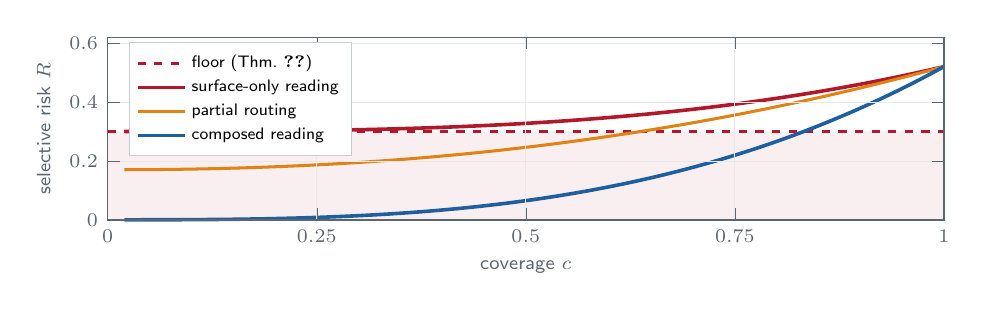
\begin{tikzpicture}
\begin{axis}[
  width=12.2cm, height=3.9cm,
  xlabel={coverage $c$}, ylabel={selective risk $R$},
  xmin=0, xmax=1.0, ymin=0, ymax=0.62,
  xtick={0,0.25,0.5,0.75,1.0}, ytick={0,0.2,0.4,0.6},
  axis line style={draw=skcSlate, line width=0.5pt},
  tick style={draw=skcSlate},
  tick label style={font=\sffamily\scriptsize, text=skcSlate},
  label style={font=\sffamily\scriptsize, text=skcSlate},
  grid=major, grid style={draw=skcMute!25, line width=0.3pt},
  axis on top, clip=false,
  legend style={font=\sffamily\fontsize{6}{7}\selectfont, draw=skcMute!55, fill=white,
                at={(0.025,0.975)}, anchor=north west, cells={anchor=west},
                row sep=-1pt, inner sep=2.5pt},
  legend image post style={line width=1pt},
]
% region no surface-gate rule can enter
\addplot[draw=none, fill=skcBlind!7, forget plot] coordinates {(0,0) (1,0) (1,0.30) (0,0.30)} \closedcycle;
\addplot[skcBlind, dashed, line width=0.8pt, domain=0:1, samples=2] {0.30};
\addlegendentry{floor (Thm.~\ref{thm:floor})}
% surface-only reading: sits on the floor, rises only near full coverage
\addplot[skcBlind, line width=1.3pt, smooth, samples=60, domain=0.02:1] {0.30+0.22*x^3};
\addlegendentry{surface-only reading}
% partial routing: intermediate plateau, own floor below the dashed line
\addplot[skcWarm, line width=1.1pt, smooth, samples=60, domain=0.02:1] {0.17+0.35*x^2.2};
\addlegendentry{partial routing}
% composed reading: descends toward zero; all three meet at full coverage
\addplot[skcCool, line width=1.3pt, smooth, samples=60, domain=0.02:1] {0.52*x^3};
\addlegendentry{composed reading}


\end{axis}
\end{tikzpicture}
\vspace{-0.4em}
\caption{\textbf{The discriminating measurement, fixed before collection.} Risk-coverage
behavior of a surface-gate rule on composed queries, read right to left as the abstention threshold
tightens. Under \textbf{surface-only reading} the curve flattens onto the floor of Theorem~\ref{thm:floor} and stops
descending, so abstaining harder buys nothing. Under \textbf{composed reading} it descends toward zero as it does
on one-hop queries. \textbf{Partial routing} descends part way, and its own floor lies below the dashed line because a
leaking gate has larger $\delta$. All three coincide at full coverage, where every rule answers
everything. \textbf{No experimental data are plotted here}, and the shapes are stated in advance so
the outcome cannot be reinterpreted afterwards. The shaded band is closed to surface-gate rules when
$\delta\approx v\approx0$.}
\label{fig:hypotheses}

\end{figure}

\section{Estimating the slack terms}
\label{app:estimation}
% =====================================================================

Two estimation points, both found by running the released smoke test on synthetic data with known
ground truth.

First, the non-negativity of $\Delta_{\mathrm{blind}}$ and $\Delta_{\mathrm{subopt}}$ in
The decomposition of Section~\ref{sec:theory} is a statement about population quantities. Both are estimated with
cross-fitted plug-ins for $R^\ast$, not the true Bayes rule, so fold-wise calibration differences can
drive an estimated term slightly negative even where the proposition holds. On synthetic data the
violations sit near a tenth of a binomial standard error. The released code therefore tolerates
violations inside sampling noise, reports them, and raises on anything larger, because a large
negative term signals an estimation fault rather than a finding. Reporting a clipped term without the
raw value would hide exactly the diagnostic that distinguishes the two.

Second, one estimation choice is wrong rather than conservative, and we record it because the mistake
is natural. Substituting the \emph{marginal} rate $\mathbb{P}(Y=1,K_2=0)$ for $v$ under-estimates the
essential supremum whenever the gate carries information about $K_1$, because shortcut answers
concentrate where the gate fires. That substitution raises the computed floor above its true value
and can manufacture an apparent violation of Theorem~\ref{thm:floor} on data where the
proposition holds. We found this by running the released smoke test on synthetic data with known
ground truth. The marginal estimator reported a violation and the conditional estimator did not, on
the same data. The released code therefore refuses the marginal estimator by default and a
regression test pins the behavior. The same applies to $\delta$, $\delta_k$, and $v_k$.

A second point concerns testing the floor empirically. Comparing the floor against the minimum of the
empirical risk-coverage curve false-alarms, because the minimum over many correlated thresholds is
biased downward and the low-coverage tail rests on few examples. We instead flag a violation only
when the one-sided upper confidence limit of the empirical risk lies strictly below the floor.

% =====================================================================
\section{Extended setup}
\label{app:setup}

\paragraph{Power.} A pre-registered minimum-detectable-effect calculation for the primary comparison
and the headline repair comparison, computed before collection rather than from the count the data
happened to provide, is a design step for the human authors and is not reported here.
% =====================================================================

\begin{center}
\small
\captionof{table}{\textbf{SKC-Bench.} F3 is the control that converts a latent entity into a written
one without changing the question. Counts are held-out items after the $K_1{=}1$ and bridge-resolved
filter, except where footnoted.}
\label{tab:bench}
\vspace{1pt}
\resizebox{\columnwidth}{!}{%
\begin{tabular}{@{}lllrl@{}}
\toprule
\textbf{Family} & \textbf{Latent entity is} & \textbf{Source} & \textbf{Items} & \textbf{Tests}\\
\midrule
F1 Bridge & the referent of a description & \citet{yang2024latent}, Wikidata & 239$^{\ddagger}$ & the base phenomenon\\
F2 Chain ($k{=}3$) & two intermediate referents & Wikidata compositions & 252$^{\ddagger}$ & compounding, Thm.~\ref{thm:floor}\\
F3 Self-written & written by the model in its own CoT & F1 with reasoning prompts & 933$^{\S}$ & whether writing restores gating\\
\bottomrule
\end{tabular}}
\vspace{1pt}
{\footnotesize $^{\ddagger}$Gemma 2 2B, layer 8, $K_1{=}1$ only (\texttt{--skip-bridge-resolution}, no
independent Patchscopes confirmation, see Section~\ref{sec:results}).
$^{\S}$Gemma 2 9B instruction-tuned, $44$ with a correct self-written bridge, $889$ with an incorrect
one.}
\vspace{-1.15em}
\end{center}


\begin{center}
\small
\captionof{table}{\textbf{Causal design.} $\uparrow$ marks a predicted change, $\approx$ no change.
See Figure~\ref{fig:causal} for what each intervention does.}
\label{tab:causal}
\vspace{1pt}
\begin{tabular}{@{}llccl@{}}
\toprule
& & \multicolumn{2}{c}{\textbf{Predicted}} &\\
\cmidrule(lr){3-4}
\textbf{Intervention} & \textbf{Read-out} & \textbf{Surface-only reading} & \textbf{Composed reading} & \textbf{What it settles}\\
\midrule
Surface steer    & refusal rate $\mid M{=}1$ & $\uparrow$   & $\approx$    & \multirow{2}{*}{is the induced refusal selective?}\\
                 & refusal rate $\mid M{=}0$ & $\uparrow$   & $\uparrow$   & \\
\addlinespace[3pt]
Bridge patch     & $\Delta$ recall           & $\downarrow$ & $\downarrow$ & \multirow{2}{*}{\textbf{decisive}, a double dissociation}\\
                 & $\Delta$ refusal rate     & $\approx$    & $\uparrow$   & \\
\addlinespace[3pt]
Gate inject      & refusal rate at bridge    & $\approx$    & $\uparrow$   & pathway absent, or present but unused\\
\addlinespace[3pt]
Graph trace      & edge weight to refusal    & $\approx 0$  & $\uparrow$   & routing as a graph property, not an inference\\
\bottomrule
\end{tabular}
\vspace{-1.15em}
\end{center}

\paragraph{Splits.} Entities are partitioned into fit and held-out sets before anything is estimated,
and the partition is by \emph{entity}, not by prompt, so that no entity appears on both sides under a
different relation. Gate directions are fit on the fit split of single-hop prompts only. Every number
reported in Section~\ref{sec:results} comes from the held-out split.

\paragraph{Gate estimators.} (i) SAE latents are selected by the separation score of
\citet{ferrando2025entity}, taking the top latent per (layer, entity type) and then the latent
maximizing the minimum separation across types, which is the generalizing choice rather than the
best-fitting one. (ii) The difference-of-means direction is the normalized difference of mean
residual-stream activations between known and unknown entity groups at the same position.
(iii) The logistic probe is $\ell_2$-regularized, with the penalty chosen by five-fold
cross-validation \emph{within} the fit split. All three are read at the final token of the entity
mention, at layer 8 for every model except Qwen3-32B (layer 24). No public SAE dictionary exists for
Llama or Qwen3, so those models use difference-of-means and probe only.

\paragraph{Interventions.} Steering coefficients are selected on a validation split disjoint from
both fit and test, following \citet{ferrando2025entity}, and reported with the sweep rather than only
the chosen value. Patching replaces the residual stream at the bridge position across a contiguous
layer window. The window is selected by the frozen-direction sweep's own empirical peak (layer,
position offset, Section~\ref{sec:res-latent}) on the composed prompt and reported, not by the
during-generation Patchscopes site, since no composed-prompt position was found where Patchscopes
decodes a clean entity.
The coefficient sweep tried on Gemma 2 2B, layer 8, is $\{-4,-2,-1,1,2,4,8\}$, and the selected
coefficient is $-4$ (maximizing validation-split refusal rate, all of which were $0.000$, so no
non-degenerate selection criterion is possible here, since refusal never varies with coefficient on
this model/template combination). The layer window is $[7,10)$, centered on that sweep's peak layer.
The same sweep on Gemma 2 9B instruction-tuned, with the layer window centered on that model's own
peak (layer 8, the same window, $[7,10)$), gives a refusal rate that is again exactly $0.000$ at every
coefficient in $\{-4,-2,-1,1,2,4,8\}$, the same degenerate outcome as the base model, evidence the
null is about this refusal template rather than about instruction tuning specifically.

\paragraph{Refusal detection.} A response counts as a refusal if it matches a refusal lexicon
\emph{and} contains no candidate attribute string. Both conditions are required, because a response
can hedge and still commit to an answer. The lexicon is fixed in advance from the validation split
and released. A held-out manual audit against the automatic label, the one place the pipeline touches
human judgment, is a task for the human authors and its agreement rate is not reported here.

\paragraph{Statistics.} All intervals are percentile bootstrap over queries with 2{,}000 resamples,
resampling queries rather than prompts so that the composed item and its decompositions move
together. AUC comparisons use both a paired bootstrap and DeLong \citep{delong1988comparing}, and we
report both, since agreement between them is evidence that neither is being driven by an artifact of
its own assumptions. Multiplicity across relation types is controlled at the 5\% level by
Benjamini-Hochberg \citep{benjamini1995controlling}. Every $\kappa$ estimate is reported at
$\alpha\in\{0.01,0.05,0.10\}$.

\paragraph{Data provenance.} Wikidata has no versioned snapshot identifier for live SPARQL queries
against \texttt{query.wikidata.org}, so we instead record the query date, which is what reproducing
the same pull requires. The two-hop query set (\texttt{data/twohop\_queries.json}) was pulled
2026-08-11, the three-hop query set (\texttt{data/threehop\_queries.json}, $n=3961$ chains) was
pulled 2026-08-26, and Wikipedia pageview counts (\texttt{data/pageviews\_twohop.json}, monthly views
summed over 2024, all 847 bridge entities from the two-hop set resolved to a real article) were
pulled 2026-08-27 from the public Wikimedia Pageviews REST API. No additional model-specific query set
was pulled beyond these three, and all reported models score against this same fixed set.

% =====================================================================

\begin{center}
\small
\captionof{table}{\textbf{All selectors, grouped by inference cost.} \emph{Audit} is the verdict of
the controlled re-run by \citet{hussain2026parallax}, where \checkmark{} exceeded chance once benchmark
artifacts were removed, $\times$ did not, and --- was not covered. Best per column within a tier is
bolded.}
\label{tab:bgr-full}
\vspace{1pt}
\resizebox{\columnwidth}{!}{%
\begin{tabular}{@{}llcccc@{}}
\toprule
\textbf{Selector} & \textbf{Cost} & \textbf{Audit} & \textbf{AUROC} $\uparrow$ &
\textbf{AURC} $\downarrow$ & \textbf{Risk @ 50\%} $\downarrow$\\
\midrule
\multicolumn{6}{@{}l}{\emph{One forward pass}}\\
\quad Surface gate \citep{ferrando2025entity}            & $1\times$ & --- & 0.562 & 0.184 & 0.160\\
\quad Semantic entropy probe \citep{kossen2024semantic}  & $1\times$ & $\times$ & 0.414 & 0.292 & 0.202\\
\addlinespace[3pt]
\multicolumn{6}{@{}l}{\emph{Extra passes or sampling}}\\
\quad $P(\text{True})$ \citep{kadavath2022know}          & $2\times$ & --- & \textbf{0.623} & 0.149 & \textbf{0.118}\\
\quad SAPLMA \citep{azaria2023internal}                  & $2\times$ & \checkmark & 0.538 & 0.167 & 0.168\\
\quad Entity-level token probes \citep{obeso2025realtime}& $2\times$ & --- & 0.565 & 0.134 & 0.134\\
\quad Lookback Lens \citep{chuang2024lookback}           & $2\times$ & --- & \textbf{0.792} & \textbf{0.089} & \textbf{0.084}\\
\quad HaloScope \citep{du2024haloscope}                  & $2\times$ & $\times$ & 0.603 & 0.156 & 0.143\\
\quad ICR probe \citep{zhang2025icrprobe}                & $2\times$ & --- & 0.518 & 0.207 & 0.160\\
\quad SelfCheckGPT \citep{manakul2023selfcheckgpt}       & $k{=}10$  & --- & 0.473 & 0.244 & 0.176\\
\quad Semantic entropy \citep{farquhar2024semantic}      & $k{=}10$  & --- & 0.575 & 0.145 & 0.143\\
\quad INSIDE \citep{chen2024inside}                      & $k{=}10$  & --- & \textbf{0.596} & \textbf{0.116} & \textbf{0.134}\\
\addlinespace[3pt]
\multicolumn{6}{@{}l}{\emph{Multi-call decomposition}}\\
\quad Self-ask abstention \citep{press2023compositionality} & multi-call & --- & 0.500 & 0.188 & 0.227\\
\quad Operadic consistency \citep{bottman2026operadic}      & multi-call & --- & 0.500 & 0.188 & 0.227\\
\midrule
\multicolumn{6}{@{}l}{\emph{Ours, one forward pass}}\\
\quad \textbf{BGR-min} (no trained parameters)           & $1\times$ & --- & 0.766 & \textbf{0.093} & \textbf{0.084}\\
\quad \textbf{BGR-lr}                                    & $1\times$ & --- & \textbf{0.781} & \textbf{0.079} & \textbf{0.076}\\
\midrule
\multicolumn{6}{@{}l}{\emph{Ceiling}}\\
\quad Oracle observing $M$                               & ---       & --- & 0.725 & 0.095 & 0.076\\
\bottomrule
\end{tabular}}

\vspace{1pt}
{\footnotesize All rows are from a real run (Gemma 2 2B, layer 8, $n{=}239$, $K_1{=}1$ only, see
Section~\ref{sec:results}). Self-ask and Operadic consistency report identical numbers because both
reduce to a constant score on this model/template. This model shows exactly $0.000$ refusal rate at
every coefficient tried (Section~\ref{sec:results}), so self-ask never abstains, and Operadic
consistency's direct-vs-decomposed answers never disagree under greedy decoding on the same
non-hedging model, a real, shared consequence of that null, not a computation error (confirmed
against two independent runs and an analytic check that only a fully constant score reproduces
AUROC$=0.500$ to this precision).}
\vspace{-1.9em}
\end{center}

\section{Prompt templates}
\label{app:prompts}
% =====================================================================

Table~\ref{tab:templates} lists the templates. They place the entity late and end on a fixed token, following \citet{tamoyan2025factual}, whose
ablation found that this form avoids the spurious correlations that arise when the prompt ends on
variable tokens. Angle brackets mark slots.

\begin{center}
\small
\captionof{table}{\textbf{Prompt templates.} The named-bridge control differs from the composed
template only in whether the bridge is written, which is the manipulation the paper turns on. It is
matched for length by padding with a type-matched modifier, so a length difference cannot explain a
gate difference.}
\label{tab:templates}
\vspace{1pt}
\begin{tabular}{@{}lp{9.4cm}@{}}
\toprule
\textbf{Role} & \textbf{Template}\\
\midrule
Single hop $j$ & \texttt{The <$r_j$> of the <type> <entity> is}\\
Composed, $k{=}2$ & \texttt{The <$r_2$> of the <$r_1$> of the <type> <$e_1$> is}\\
Composed, $k{=}3$ & \texttt{The <$r_3$> of the <$r_2$> of the <$r_1$> of the <type> <$e_1$> is}\\
Named-bridge control & \texttt{The <$r_2$> of the <type$_2$> <$b$> is}\\
Chain of thought (F3) & \texttt{Answer step by step. The <$r_2$> of the <$r_1$> of the <type>
<$e_1$> is}\\
\bottomrule
\end{tabular}
\vspace{-1.15em}
\end{center}

\paragraph{Screening.} Before use, every template is screened for spurious correlation. We replace
the entity with a type-matched placeholder that carries no identity (for example a randomly generated
name of matched token length) and confirm that gate separation collapses to chance. A template on
which separation survives entity replacement is measuring the template, not the entity, and is
discarded. This screening has not yet been run against the templates in Table~\ref{tab:templates}, and
reporting which templates survive and their separation scores before and after replacement is a
task for the human authors before submission.

\paragraph{Relations.} Relations are drawn from the entity types used by \citet{ferrando2025entity},
with composable pairs chosen so that the bridge is itself an entity with its own attributes. We
exclude relations whose answers are non-textual or ambiguous in modality, such as coordinates,
following the same exclusion made by \citet{tamoyan2025factual}. The released two-hop set
(\texttt{data/twohop\_queries.json}) uses one composable pair, entity type \emph{player}, place of
birth $\to$ country. The released three-hop set (\texttt{data/threehop\_queries.json}) uses one
composable triple, the same entity type, place of birth $\to$ country $\to$ continent. This is a
disclosed limitation, not a design choice presented as broader than it is. The released Ferrando et
al.\ data yields a usable two-hop bridge for only this one entity-type pair (Appendix~\ref{app:setup}'s
own data-provenance note), so the relation inventory does not span every entity type this pipeline
otherwise supports.

% =====================================================================
\section{Use of large language models}
\label{app:ai}
% =====================================================================

ICLR requires disclosure of AI use. This section is not counted toward the page limit.

In this work we used generative AI tools to help develop the conceptual framework, formulate the
mathematical claims and assist in writing the proofs in Appendix~\ref{app:proofs}, propose and refine
the hypotheses in Section~\ref{sec:hypotheses}, and give feedback on the experimental design in
Section~\ref{sec:causal-design}. We also used them to search and summarize related literature, to
draft parts of the manuscript, to create figures, and to write analysis code.

We have reviewed all AI-assisted work. We take responsibility for
the final content of this work, including all text, claims, and artifacts produced with the aid of
generative AI. The authors are the sole authors of this paper.

\end{document}
